\section{DIL\_\-Topical\_\-List  Class Reference}
\label{classDIL__Topical__List}\index{DIL_Topical_List@{DIL\_\-Topical\_\-List}}
{\tt \#include $<$dil2al.hh$>$}

Inheritance diagram for DIL\_\-Topical\_\-List::\begin{figure}[H]
\begin{center}
\leavevmode
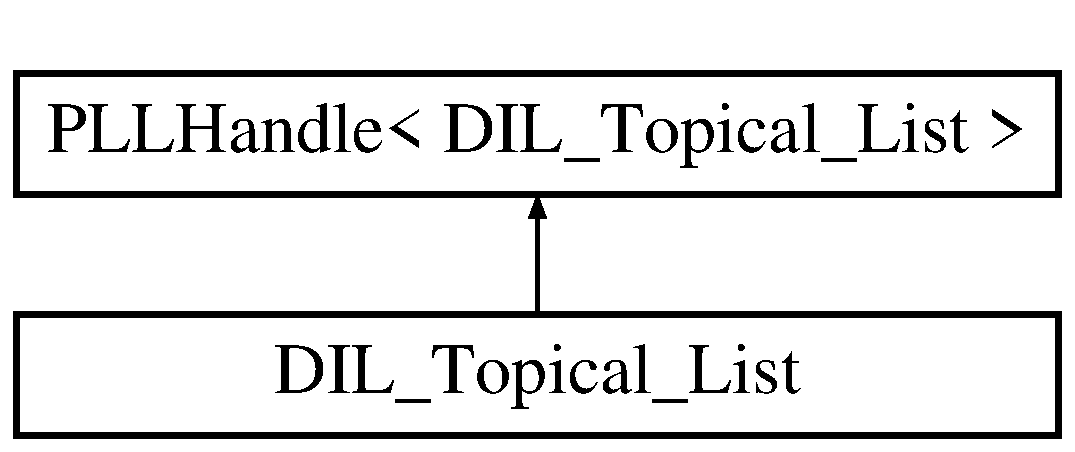
\includegraphics[height=2cm]{classDIL__Topical__List}
\end{center}
\end{figure}
\subsection*{Public Methods}
\begin{CompactItemize}
\item 
{\bf DIL\_\-Topical\_\-List} ({\bf DIL\_\-entry} \&e)
\item 
{\bf DIL\_\-Topical\_\-List} ({\bf DIL\_\-entry} \&e, {\bf String} tfile, {\bf String} ttitle, float trelevance)
\item 
{\bf $\sim$DIL\_\-Topical\_\-List} ()
\item 
bool {\bf Write\_\-to\_\-Binary\_\-Cache} (ofstream \&cfl)
\item 
bool {\bf Read\_\-from\_\-Binary\_\-Cache} (ifstream \&cfl)
\item 
bool {\bf Binary\_\-Cache\_\-Diagnostic} (DIL\_\-Topical\_\-List $\ast$cached, int \&testedbytes)
\end{CompactItemize}
\subsection*{Public Attributes}
\begin{CompactItemize}
\item 
{\bf filetitle\_\-t} {\bf dil}
\item 
float {\bf relevance}
\end{CompactItemize}
\subsection*{Protected Attributes}
\begin{CompactItemize}
\item 
{\bf DIL\_\-entry} $\ast$ {\bf entry}
\end{CompactItemize}


\subsection{Constructor \& Destructor Documentation}
\index{DIL_Topical_List@{DIL\_\-Topical\_\-List}!DIL_Topical_List@{DIL\_\-Topical\_\-List}}
\index{DIL_Topical_List@{DIL\_\-Topical\_\-List}!DIL_Topical_List@{DIL\_\-Topical\_\-List}}
\subsubsection{\setlength{\rightskip}{0pt plus 5cm}DIL\_\-Topical\_\-List::DIL\_\-Topical\_\-List ({\bf DIL\_\-entry} \& {\em e})}\label{classDIL__Topical__List_a0}




Definition at line 679 of file utilities.cc.



\footnotesize\begin{verbatim}679 : entry(&e), relevance(0.0) {}
\end{verbatim}\normalsize 
\index{DIL_Topical_List@{DIL\_\-Topical\_\-List}!DIL_Topical_List@{DIL\_\-Topical\_\-List}}
\index{DIL_Topical_List@{DIL\_\-Topical\_\-List}!DIL_Topical_List@{DIL\_\-Topical\_\-List}}
\subsubsection{\setlength{\rightskip}{0pt plus 5cm}DIL\_\-Topical\_\-List::DIL\_\-Topical\_\-List ({\bf DIL\_\-entry} \& {\em e}, {\bf String} {\em tfile}, {\bf String} {\em ttitle}, float {\em trelevance})}\label{classDIL__Topical__List_a1}




Definition at line 681 of file utilities.cc.

References dil, filetitle\_\-t::file, and filetitle\_\-t::title.



\footnotesize\begin{verbatim}681                                                                                               : entry(&e), relevance(trelevance) {
682         dil.file = tfile;
683         dil.title = ttitle;
684 }
\end{verbatim}\normalsize 
\index{DIL_Topical_List@{DIL\_\-Topical\_\-List}!~DIL_Topical_List@{$\sim$DIL\_\-Topical\_\-List}}
\index{~DIL_Topical_List@{$\sim$DIL\_\-Topical\_\-List}!DIL_Topical_List@{DIL\_\-Topical\_\-List}}
\subsubsection{\setlength{\rightskip}{0pt plus 5cm}DIL\_\-Topical\_\-List::$\sim$DIL\_\-Topical\_\-List ()\hspace{0.3cm}{\tt  [inline]}}\label{classDIL__Topical__List_a2}




Definition at line 529 of file dil2al.hh.



\footnotesize\begin{verbatim}529 {} 
\end{verbatim}\normalsize 


\subsection{Member Function Documentation}
\index{DIL_Topical_List@{DIL\_\-Topical\_\-List}!Binary_Cache_Diagnostic@{Binary\_\-Cache\_\-Diagnostic}}
\index{Binary_Cache_Diagnostic@{Binary\_\-Cache\_\-Diagnostic}!DIL_Topical_List@{DIL\_\-Topical\_\-List}}
\subsubsection{\setlength{\rightskip}{0pt plus 5cm}bool DIL\_\-Topical\_\-List::Binary\_\-Cache\_\-Diagnostic (DIL\_\-Topical\_\-List $\ast$ {\em cached}, int \& {\em testedbytes})}\label{classDIL__Topical__List_a5}




Definition at line 722 of file utilities.cc.

References dil, entry, filetitle\_\-t::file, relevance, filetitle\_\-t::title, and VOUT.

Referenced by DIL\_\-entry\_\-parameters::Binary\_\-Cache\_\-Diagnostic().



\footnotesize\begin{verbatim}722                                                                                            {
723   // test if the quick load cache process works reliably
724   // this is the original Topical_List, cached is the one retrieved from the binary cache
725   //   start of this object test
726   int localtestedbytes = sizeof(PLLHandle<DIL_Topical_List>);
727   if ((*entry)!=(*(cached->entry))) VOUT << "*** DIL_Topical_List entry mismatch\n"; // testing if DIL_ID==DIL_ID
728   localtestedbytes += sizeof(entry);
729   if (dil.file!=cached->dil.file) VOUT << "*** DIL_Topical_List dil.file mismatch\n";
730   if (dil.title!=cached->dil.title) VOUT << "*** DIL_Topical_List dil.title mismatch\n";
731   localtestedbytes += sizeof(dil);
732   if (relevance!=cached->relevance) VOUT << "*** DIL_Topical_List relevance mismatch\n";
733   localtestedbytes += sizeof(relevance);
734   //   end of this object test
735   if (localtestedbytes!=sizeof(DIL_Topical_List)) VOUT << "*** testedbytes!=sizeof(DIL_Topical_List)\n";
736   testedbytes += localtestedbytes;
737   return true;
738 }
\end{verbatim}\normalsize 
\index{DIL_Topical_List@{DIL\_\-Topical\_\-List}!Read_from_Binary_Cache@{Read\_\-from\_\-Binary\_\-Cache}}
\index{Read_from_Binary_Cache@{Read\_\-from\_\-Binary\_\-Cache}!DIL_Topical_List@{DIL\_\-Topical\_\-List}}
\subsubsection{\setlength{\rightskip}{0pt plus 5cm}bool DIL\_\-Topical\_\-List::Read\_\-from\_\-Binary\_\-Cache (ifstream \& {\em cfl})}\label{classDIL__Topical__List_a4}




Definition at line 700 of file utilities.cc.

References dil, filetitle\_\-t::file, READSOMETYPE, relevance, TEST\_\-LBUF\_\-BOUNDS, and filetitle\_\-t::title.

Referenced by DIL\_\-entry\_\-parameters::Read\_\-from\_\-Binary\_\-Cache().



\footnotesize\begin{verbatim}700                                                             {
701   const int LLEN = 1024;
702   char lbuf[LLEN];
703   // dil.file
704   int dilfilelen;
705   if ((cfl.read((READSOMETYPE) (&dilfilelen), sizeof(dilfilelen))).gcount()<sizeof(dilfilelen)) return false;
706   TEST_LBUF_BOUNDS(dilfilelen,"DIL_Topical_List::Read_from_Binary_Cache()")
707   if ((cfl.read((READSOMETYPE) lbuf, dilfilelen)).gcount()<dilfilelen) return false;
708   lbuf[dilfilelen]='\0';
709   dil.file = lbuf;
710   // dil.title
711   int diltitlelen;
712   if ((cfl.read((READSOMETYPE) (&diltitlelen), sizeof(diltitlelen))).gcount()<sizeof(diltitlelen)) return false;
713   TEST_LBUF_BOUNDS(diltitlelen,"DIL_Topical_List::Read_from_Binary_Cache()")
714   if ((cfl.read((READSOMETYPE) lbuf, diltitlelen)).gcount()<diltitlelen) return false;
715   lbuf[diltitlelen]='\0';
716   dil.title = lbuf;
717   // relevance
718   if ((cfl.read((READSOMETYPE) (&relevance), sizeof(relevance))).gcount()<sizeof(relevance)) return false;
719   return true;
720 }
\end{verbatim}\normalsize 
\index{DIL_Topical_List@{DIL\_\-Topical\_\-List}!Write_to_Binary_Cache@{Write\_\-to\_\-Binary\_\-Cache}}
\index{Write_to_Binary_Cache@{Write\_\-to\_\-Binary\_\-Cache}!DIL_Topical_List@{DIL\_\-Topical\_\-List}}
\subsubsection{\setlength{\rightskip}{0pt plus 5cm}bool DIL\_\-Topical\_\-List::Write\_\-to\_\-Binary\_\-Cache (ofstream \& {\em cfl})}\label{classDIL__Topical__List_a3}




Definition at line 686 of file utilities.cc.

References String::chars(), dil, filetitle\_\-t::file, String::length(), relevance, and filetitle\_\-t::title.



\footnotesize\begin{verbatim}686                                                            {
687   // dil.file
688   int dilfilelen = dil.file.length();
689   cfl.write((const void *) (&dilfilelen), sizeof(dilfilelen));
690   cfl.write((const void *) dil.file.chars(), dilfilelen);
691   // dil.title
692   int diltitlelen = dil.title.length();
693   cfl.write((const void *) (&diltitlelen), sizeof(diltitlelen));
694   cfl.write((const void *) dil.title.chars(), diltitlelen);
695   // relevance
696   cfl.write((const void *) (&relevance), sizeof(relevance));
697   return true;
698 }
\end{verbatim}\normalsize 


\subsection{Member Data Documentation}
\index{DIL_Topical_List@{DIL\_\-Topical\_\-List}!dil@{dil}}
\index{dil@{dil}!DIL_Topical_List@{DIL\_\-Topical\_\-List}}
\subsubsection{\setlength{\rightskip}{0pt plus 5cm}{\bf filetitle\_\-t} DIL\_\-Topical\_\-List::dil}\label{classDIL__Topical__List_m0}




Definition at line 531 of file dil2al.hh.

Referenced by Binary\_\-Cache\_\-Diagnostic(), DIL\_\-Topical\_\-List(), generate\_\-AL(), Active\_\-List::generate\_\-focused\_\-AL(), Detailed\_\-Items\_\-List::Get\_\-All\_\-DIL\_\-ID\_\-File\_\-Parameters(), Read\_\-from\_\-Binary\_\-Cache(), DIL\_\-Visualize\_\-with\_\-FORM\_\-Tabs::Visualize\_\-Element(), DIL\_\-Visualize\_\-with\_\-HTML\_\-Tabs::Visualize\_\-Element(), and Write\_\-to\_\-Binary\_\-Cache().\index{DIL_Topical_List@{DIL\_\-Topical\_\-List}!entry@{entry}}
\index{entry@{entry}!DIL_Topical_List@{DIL\_\-Topical\_\-List}}
\subsubsection{\setlength{\rightskip}{0pt plus 5cm}{\bf DIL\_\-entry}$\ast$ DIL\_\-Topical\_\-List::entry\hspace{0.3cm}{\tt  [protected]}}\label{classDIL__Topical__List_n0}




Definition at line 523 of file dil2al.hh.

Referenced by Binary\_\-Cache\_\-Diagnostic().\index{DIL_Topical_List@{DIL\_\-Topical\_\-List}!relevance@{relevance}}
\index{relevance@{relevance}!DIL_Topical_List@{DIL\_\-Topical\_\-List}}
\subsubsection{\setlength{\rightskip}{0pt plus 5cm}float DIL\_\-Topical\_\-List::relevance}\label{classDIL__Topical__List_m1}




Definition at line 532 of file dil2al.hh.

Referenced by Binary\_\-Cache\_\-Diagnostic(), Detailed\_\-Items\_\-List::Get\_\-All\_\-DIL\_\-ID\_\-File\_\-Parameters(), Read\_\-from\_\-Binary\_\-Cache(), and Write\_\-to\_\-Binary\_\-Cache().

The documentation for this class was generated from the following files:\begin{CompactItemize}
\item 
{\bf dil2al.hh}\item 
{\bf utilities.cc}\end{CompactItemize}
